\documentclass[11pt,a4paper]{article}
\usepackage[utf8]{inputenc}
\usepackage[margin=1in]{geometry}
\usepackage{amsmath,amsfonts,amssymb}
\usepackage{graphicx}
\usepackage{tikz}
\usepackage{pgfgantt}
\usepackage{booktabs}
\usepackage{array}
\usepackage{enumitem}
\usepackage{float}
\usepackage{xcolor}
\usepackage{hyperref}
\usepackage{fancyhdr}
\usepackage{titlesec}

% Colors
\definecolor{bankBlue}{RGB}{0,123,255}
\definecolor{bankLightBlue}{RGB}{52,152,219}
\definecolor{bankGreen}{RGB}{40,167,69}
\definecolor{bankOrange}{RGB}{255,193,7}

% Header and footer
\pagestyle{fancy}
\fancyhf{}
\fancyhead[L]{Campus Management System - Project Document}
\fancyhead[R]{Version 1.0}
\fancyfoot[C]{\thepage}

% Title formatting
\titleformat{\section}{\Large\bfseries\color{bankBlue}}{\thesection}{1em}{}
\titleformat{\subsection}{\large\bfseries\color{bankLightBlue}}{\thesubsection}{1em}{}
\titleformat{\subsubsection}{\normalsize\bfseries\color{bankBlue}}{\thesubsubsection}{1em}{}

% Hyperlink setup
\hypersetup{
    colorlinks=true,
    linkcolor=bankBlue,
    urlcolor=bankOrange,
    citecolor=bankLightBlue
}

\begin{document}

% Title page
\begin{titlepage}
\centering
\vspace*{2cm}

{\Huge\bfseries\color{bankBlue} Campus Management System}\\[0.5cm]
{\Large Full-Stack CRUD Application Project Document}\\[2cm]

\begin{tabular}{ll}
\textbf{Assignment:} & Final Project - Full-Stack CRUD Application (Campus Management System) \\
\textbf{Start Date:} & November 18, 2025 \\
\textbf{Due Date:} & December 12, 2025, 11:59 PM \\
\textbf{Project Duration:} & 4 weeks \\
\textbf{Team Size:} & 2 developers (David \& Kevin) \\
\textbf{Document Version:} & 1.0 \\
\textbf{Last Updated:} & December 2, 2025 \\
\end{tabular}

\vfill

{\large A PERN-based Campus Management System with CRUD functionality for campuses and students, client-side routing, and Redux state management.}

\end{titlepage}

% Table of Contents
\tableofcontents
\newpage

\section{Feature Requirements}

\subsection{Core Functional Views}

\subsubsection{Home Page View}
\begin{itemize}[leftmargin=*]
    \item \textbf{Default Landing}: Users land on a visually pleasing home page by default.
    \item \textbf{Navigation}: Clear navigation options to access All Campuses and All Students views.
    \item \textbf{Branding}: Campus Management System title and brief description of the system.
\end{itemize}

\subsubsection{All Campuses View}
\begin{itemize}[leftmargin=*]
    \item \textbf{Campus List}: Display a list of all campuses, including at least campus name and image.
    \item \textbf{Empty State}: Show an informative message when no campuses exist.
    \item \textbf{Add Campus}: Provide a button/link to navigate to the Add Campus View.
    \item \textbf{Delete Campus}: Allow deletion of a campus via a button (either here or from Single Campus View).
    \item \textbf{Navigation}: Clicking a campus name navigates to the Single Campus View.
\end{itemize}

\subsubsection{Single Campus View}
\begin{itemize}[leftmargin=*]
    \item \textbf{Campus Details}: Show campus name, image, address, and description.
    \item \textbf{Enrolled Students}: Display a list of enrolled students' names, or a helpful message if none exist.
    \item \textbf{Student Navigation}: Clicking a student name navigates to that student's Single Student View.
    \item \textbf{Student Management}: Support adding new/existing students to the campus and removing students from the campus.
    \item \textbf{Campus Management}: Provide navigation to the Edit Campus View and an option to delete the campus.
\end{itemize}

\subsubsection{Add Campus View}
\begin{itemize}[leftmargin=*]
    \item \textbf{Form Inputs}: Fields for name, address, description, and image URL.
    \item \textbf{Validation}: Real-time validation with helpful error messages.
    \item \textbf{Persistence}: On valid submission, the new campus is persisted to the database and appears in the All Campuses View without a page refresh.
\end{itemize}

\subsubsection{Edit Campus View}
\begin{itemize}[leftmargin=*]
    \item \textbf{Pre-filled Form}: Existing campus information loaded into editable fields.
    \item \textbf{Form Inputs}: Fields for name, address, description, and image URL.
    \item \textbf{Validation}: Real-time validation similar to Add Campus View.
    \item \textbf{Update Behavior}: On valid submission, the campus is updated in the database and the UI reflects changes without a full page reload.
\end{itemize}

\subsubsection{All Students View}
\begin{itemize}[leftmargin=*]
    \item \textbf{Student List}: Display all students, including at least full name.
    \item \textbf{Empty State}: Show an informative message when no students exist.
    \item \textbf{Add Student}: Provide a button/link to navigate to the Add Student View.
    \item \textbf{Delete Student}: Allow deletion of a student via a button (either here or from Single Student View).
    \item \textbf{Navigation}: Clicking a student name navigates to the Single Student View.
\end{itemize}

\subsubsection{Single Student View}
\begin{itemize}[leftmargin=*]
    \item \textbf{Student Details}: Show full name, email, image, and GPA.
    \item \textbf{Campus Info}: Display the name of the student's campus, or a message if not enrolled.
    \item \textbf{Navigation}: Link to navigate to the student's campus Single Campus View.
    \item \textbf{Student Management}: Provide navigation to Edit Student View and an option to delete the student.
\end{itemize}

\subsubsection{Add Student View}
\begin{itemize}[leftmargin=*]
    \item \textbf{Form Inputs}: Fields for first name, last name, email, image URL, GPA, and optionally campus.
    \item \textbf{Validation}: Real-time validation for required fields, email format, and GPA range (0.0--4.0).
    \item \textbf{Persistence}: On valid submission, the new student is persisted and appears in All Students View without a page refresh.
\end{itemize}

\subsubsection{Edit Student View}
\begin{itemize}[leftmargin=*]
    \item \textbf{Pre-filled Form}: Existing student data loaded for editing.
    \item \textbf{Form Inputs}: Fields for first name, last name, email, image URL, GPA, and campus selection.
    \item \textbf{Validation}: Real-time validation consistent with Add Student View.
    \item \textbf{Update Behavior}: On submission, the student is updated in the database and the UI reflects the changes immediately.
\end{itemize}

\subsection{Technical Requirements}

\subsubsection{UI (React)}
\begin{itemize}[leftmargin=*]
    \item \textbf{All Campuses Component}: Displays list of campuses with name and image.
    \item \textbf{All Students Component}: Displays list of students with at least student name.
    \item \textbf{Single Campus Component}: Displays details for one campus and its students.
    \item \textbf{Single Student Component}: Displays details for one student and their campus.
    \item \textbf{Form Components}: Reusable form patterns for add/edit campus and add/edit student views with inline validation.
\end{itemize}

\subsubsection{Client-Side Routing (React Router)}
\begin{itemize}[leftmargin=*]
    \item \textbf{Route Definitions}:
    \begin{itemize}
        \item \texttt{/} -- Home page.
        \item \texttt{/campuses} -- All Campuses View.
        \item \texttt{/students} -- All Students View.
        \item \texttt{/campus/:campusId} -- Single Campus View.
        \item \texttt{/student/:studentId} -- Single Student View.
        \item \texttt{/campuses/new} -- Add Campus View.
        \item \texttt{/students/new} -- Add Student View.
        \item \texttt{/campuses/:campusId/edit} -- Edit Campus View.
        \item \texttt{/students/:studentId/edit} -- Edit Student View.
    \end{itemize}
    \item \textbf{Navigation}: Header navigation links to Home, All Campuses, and All Students.
    \item \textbf{Deep Linking}: Direct URL access to any supported route.
\end{itemize}

\subsubsection{State Management (Redux)}
\begin{itemize}[leftmargin=*]
    \item \textbf{Campuses Reducer}: Manages the collection and loading/error states for campuses.
    \item \textbf{Students Reducer}: Manages the collection and loading/error states for students.
    \item \textbf{Thunks}: Asynchronous action creators for fetching, creating, updating, and deleting campuses and students.
    \item \textbf{Global Store}: Single Redux store combining campus and student reducers, integrated with React via Provider.
\end{itemize}

\subsubsection{Database (PostgreSQL via Sequelize)}
\begin{itemize}[leftmargin=*]
    \item \textbf{Campus Model}:
    \begin{itemize}
        \item \texttt{name}: non-null, non-empty string.
        \item \texttt{address}: non-null, non-empty string.
        \item \texttt{description}: text, nullable.
        \item \texttt{imageUrl}: string with default image URL, nullable.
    \end{itemize}
    \item \textbf{Student Model}:
    \begin{itemize}
        \item \texttt{firstName}: non-null, non-empty string.
        \item \texttt{lastName}: non-null, non-empty string.
        \item \texttt{email}: non-null, non-empty string with validation.
        \item \texttt{imageUrl}: string with default image URL, nullable.
        \item \texttt{gpa}: decimal between 0.0 and 4.0, nullable.
    \end{itemize}
    \item \textbf{Associations}:
    \begin{itemize}
        \item One Campus has many Students.
        \item One Student belongs to at most one Campus.
    \end{itemize}
\end{itemize}

\subsubsection{API / Server-Side Routing (Express + Sequelize)}
\begin{itemize}[leftmargin=*]
    \item \textbf{All Resources}:
    \begin{itemize}
        \item \texttt{GET /api/students} -- all students.
        \item \texttt{GET /api/campuses} -- all campuses.
    \end{itemize}
    \item \textbf{Single Resources}:
    \begin{itemize}
        \item \texttt{GET /api/students/:id} -- single student including campus.
        \item \texttt{GET /api/campuses/:id} -- single campus including students.
    \end{itemize}
    \item \textbf{Create}:
    \begin{itemize}
        \item \texttt{POST /api/students} -- add a new student.
        \item \texttt{POST /api/campuses} -- add a new campus.
    \end{itemize}
    \item \textbf{Update}:
    \begin{itemize}
        \item \texttt{PUT /api/students/:id} -- edit existing student.
        \item \texttt{PUT /api/campuses/:id} -- edit existing campus.
    \end{itemize}
    \item \textbf{Delete}:
    \begin{itemize}
        \item \texttt{DELETE /api/students/:id} -- delete student.
        \item \texttt{DELETE /api/campuses/:id} -- delete campus.
    \end{itemize}
\end{itemize}

\subsection{Version Control and Code Quality Requirements}
\begin{itemize}[leftmargin=*]
    \item \textbf{Git Workflow}: Use feature branches, pull requests, and small, descriptive commits.
    \item \textbf{Code Organization}: Keep code modular, well-formatted, and commented.
    \item \textbf{Documentation}: README files for both front-end and back-end list team members and GitHub usernames.
\end{itemize}

\section{Application Architecture Description and Diagram}

\subsection{Architecture Overview}

The Campus Management System follows a \textbf{PERN (PostgreSQL, Express, React, Node.js) full-stack architecture} based on the assignment specification in \href{file:///c%3A/Users/darkf/Documents/Campus-Management-System/Final_Project_Full_Stack_CRUD_Application_v2_1_Fall_2025.pdf}{the project PDF}. The backend exposes a RESTful API for managing campuses and students, while the frontend is a \textbf{React Single-Page Application (SPA)} using React Router and Redux. The architecture emphasizes \textbf{separation of concerns}, \textbf{unidirectional data flow}, and \textbf{scalable CRUD operations}.

\subsection{System Components}

\subsubsection{Presentation Layer (React Components)}
\begin{itemize}[leftmargin=*]
    \item \textbf{HomePageView}: Default landing page with navigation to main views.
    \item \textbf{AllCampusesView}: Displays the list of campuses.
    \item \textbf{CampusView}: Displays a single campus and its enrolled students.
    \item \textbf{NewCampusView}: Form for adding a new campus.
    \item \textbf{EditCampusView}: Form for editing an existing campus.
    \item \textbf{AllStudentsView}: Displays the list of students.
    \item \textbf{StudentView}: Displays a single student's details.
    \item \textbf{NewStudentView}: Form for adding a new student.
    \item \textbf{EditStudentView}: Form for editing an existing student.
\end{itemize}

\subsubsection{Routing Layer (React Router)}
\begin{itemize}[leftmargin=*]
    \item \textbf{Router}: \texttt{BrowserRouter} wraps the entire React application.
    \item \textbf{Routes}: Map URL paths to campus and student views.
    \item \textbf{Navigation}: \texttt{Link} components used for navigating between views.
    \item \textbf{Error Handling}: Fallback route for invalid URLs (e.g., 404 view).
\end{itemize}

\subsubsection{State Management Layer (Redux Store)}
\begin{itemize}[leftmargin=*]
    \item \textbf{Campuses Slice}:
    \begin{itemize}
        \item \texttt{campuses}: Array of campus objects.
        \item \texttt{selectedCampus}: Detailed campus for Single Campus View.
        \item \texttt{status}: Loading/error statuses.
    \end{itemize}
    \item \textbf{Students Slice}:
    \begin{itemize}
        \item \texttt{students}: Array of student objects.
        \item \texttt{selectedStudent}: Detailed student for Single Student View.
        \item \texttt{status}: Loading/error statuses.
    \end{itemize}
\end{itemize}

\subsubsection{Business Logic Layer}
\begin{itemize}[leftmargin=*]
    \item \textbf{CRUD Operations}: Thunks encapsulate create, read, update, and delete logic for both campuses and students.
    \item \textbf{Validation}: Shared validation utilities enforce constraints such as GPA range and required fields.
    \item \textbf{Association Management}: Logic for assigning and unassigning students to/from campuses.
    \item \textbf{Error Handling}: Graceful user feedback on API failures.
\end{itemize}

\subsection{Architecture Diagram}

\begin{figure}[h]
\centering
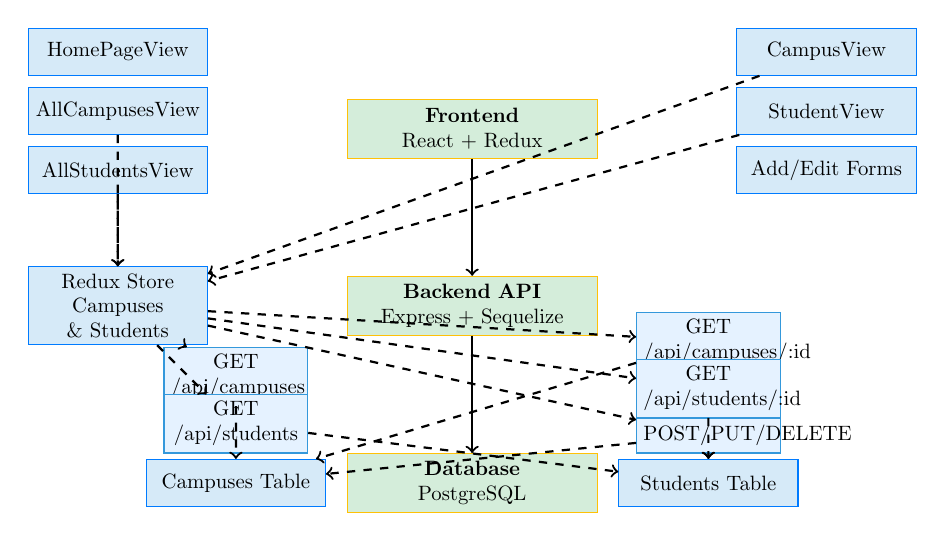
\begin{tikzpicture}[
    box/.style={rectangle, draw=bankBlue, fill=bankLightBlue!20, text width=2.8cm, text centered, minimum height=0.8cm},
    layer/.style={rectangle, draw=bankOrange, fill=bankGreen!20, text width=4cm, text centered, minimum height=1cm},
    small/.style={rectangle, draw=bankLightBlue, fill=bankBlue!10, text width=2.2cm, text centered, minimum height=0.5cm},
    scale=0.75,
    transform shape
]

% Main Layers
\node[layer] (frontend) at (0,7.5) {\textbf{Frontend}\\React + Redux};
\node[layer] (backend)  at (0,4.5) {\textbf{Backend API}\\Express + Sequelize};
\node[layer] (db)       at (0,1.5) {\textbf{Database}\\PostgreSQL};

% Frontend Components
\node[box] (home)      at (-6,8.8) {HomePageView};
\node[box] (acamp)     at (-6,7.8) {AllCampusesView};
\node[box] (astud)     at (-6,6.8) {AllStudentsView};
\node[box] (camp)      at (6,8.8)  {CampusView};
\node[box] (stud)      at (6,7.8)  {StudentView};
\node[box] (forms)     at (6,6.8)  {Add/Edit Forms};

% Redux Store
\node[box] (store)     at (-6,4.5) {Redux Store\\Campuses \& Students};

% Backend API Endpoints
\node[small] (apiCampAll)  at (-4,3.3) {GET /api/campuses};
\node[small] (apiStudAll)  at (-4,2.5) {GET /api/students};
\node[small] (apiCampOne)  at (4,3.9) {GET /api/campuses/:id};
\node[small] (apiStudOne)  at (4,3.1) {GET /api/students/:id};
\node[small] (apiMut)      at (4,2.3) {POST/PUT/DELETE};

% Database Tables
\node[box] (campTable) at (-4,1.5) {Campuses Table};
\node[box] (studTable) at (4,1.5)  {Students Table};

% Main Connections
\draw[->, thick] (frontend) -- (backend);
\draw[->, thick] (backend) -- (db);

% Frontend to Store
\draw[->, thick, dashed] (acamp) -- (store);
\draw[->, thick, dashed] (astud) -- (store);
\draw[->, thick, dashed] (camp) -- (store);
\draw[->, thick, dashed] (stud) -- (store);

% Store to Backend
\draw[->, thick, dashed] (store) -- (apiCampAll);
\draw[->, thick, dashed] (store) -- (apiStudAll);
\draw[->, thick, dashed] (store) -- (apiCampOne);
\draw[->, thick, dashed] (store) -- (apiStudOne);
\draw[->, thick, dashed] (store) -- (apiMut);

% Backend to DB
\draw[->, thick, dashed] (apiCampAll) -- (campTable);
\draw[->, thick, dashed] (apiCampOne) -- (campTable);
\draw[->, thick, dashed] (apiStudAll) -- (studTable);
\draw[->, thick, dashed] (apiStudOne) -- (studTable);
\draw[->, thick, dashed] (apiMut) -- (campTable);
\draw[->, thick, dashed] (apiMut) -- (studTable);

\end{tikzpicture}
\caption{Campus Management System Application Architecture}
\end{figure}

\subsection{Data Flow}

\begin{enumerate}[leftmargin=*]
    \item \textbf{User Navigation}: User navigates to a view (e.g., All Campuses, Single Student) via header links or deep links.
    \item \textbf{Route Matching}: React Router matches the URL path to a route and renders the correct view component.
    \item \textbf{State Initialization}: Components dispatch Redux thunks to fetch initial data from the backend API.
    \item \textbf{Backend Processing}: Express routes handle requests, interact with Sequelize models, and query/update PostgreSQL.
    \item \textbf{Response Handling}: The backend responds with JSON data, which Redux reducers use to update the store.
    \item \textbf{UI Update}: React components re-render with the latest state, reflecting changes without a page reload.
    \item \textbf{Subsequent Actions}: User-initiated CRUD actions (add, edit, delete) follow the same flow through thunks and reducers.
\end{enumerate}

\subsection{Technology Stack}

\begin{itemize}[leftmargin=*]
    \item \textbf{React}: Component-based UI library for building the SPA.
    \item \textbf{React Router}: Client-side routing for navigation between views.
    \item \textbf{Redux}: State management for campuses and students.
    \item \textbf{Node.js}: Runtime environment for the backend server.
    \item \textbf{Express}: Web framework for building RESTful API endpoints.
    \item \textbf{PostgreSQL}: Relational database for persistent data storage.
    \item \textbf{Sequelize}: ORM layer for interacting with PostgreSQL.
    \item \textbf{Git \& GitHub}: Version control and repository hosting.
\end{itemize}

\subsection{Key Design Patterns}

\begin{itemize}[leftmargin=*]
    \item \textbf{Component Composition}: Break UI into reusable, focused components (views and containers).
    \item \textbf{Container/Presentational Split}: Containers handle data fetching and state, while views focus on layout and styling.
    \item \textbf{Unidirectional Data Flow}: Redux ensures predictable state updates with actions and reducers.
    \item \textbf{Separation of Concerns}: Backend API, database models, and frontend UI remain decoupled.
    \item \textbf{Validation and Error Handling}: Centralized validation logic to keep components simple and robust.
\end{itemize}

\section{Epics, User Stories, and Acceptance Criteria}

\subsection{Epic 1: Home Page and Navigation}

\subsubsection{User Story 1.1: Home Page Navigation}
\textbf{As a} user\\
\textbf{I want to} land on a home page with clear navigation\\
\textbf{So that} I can easily access campuses and students

\textbf{Acceptance Criteria:}
\begin{itemize}[leftmargin=*]
    \item Home page is rendered at route \texttt{/}.
    \item Page clearly presents links or buttons to All Campuses and All Students views.
    \item Navigation uses React Router \texttt{Link} components.
    \item Design is visually appealing and responsive.
\end{itemize}

\subsection{Epic 2: All Campuses Management}

\subsubsection{User Story 2.1: View All Campuses}
\textbf{As a} user\\
\textbf{I want to} see a list of all campuses\\
\textbf{So that} I can browse the available campuses

\textbf{Acceptance Criteria:}
\begin{itemize}[leftmargin=*]
    \item Route \texttt{/campuses} displays All Campuses View.
    \item Each campus card shows at least campus name and image.
    \item If no campuses exist, an informative message is displayed.
    \item Clicking a campus name navigates to its Single Campus View.
\end{itemize}

\subsubsection{User Story 2.2: Add Campus from All Campuses View}
\textbf{As a} user\\
\textbf{I want to} add a new campus from the All Campuses View\\
\textbf{So that} I can grow the list of campuses

\textbf{Acceptance Criteria:}
\begin{itemize}[leftmargin=*]
    \item A button or link navigates to the Add Campus View.
    \item After successfully creating a campus, the All Campuses list updates without a full page refresh.
\end{itemize}

\subsubsection{User Story 2.3: Delete Campus}
\textbf{As a} user\\
\textbf{I want to} delete a campus\\
\textbf{So that} I can remove campuses that are no longer active

\textbf{Acceptance Criteria:}
\begin{itemize}[leftmargin=*]
    \item Each campus has an accessible Delete button (in All Campuses or Single Campus View).
    \item Clicking Delete sends a request to remove the campus from the database.
    \item The campus disappears from the list without requiring a page reload.
\end{itemize}

\subsection{Epic 3: Single Campus Management}

\subsubsection{User Story 3.1: View Single Campus Details}
\textbf{As a} user\\
\textbf{I want to} view details about a specific campus\\
\textbf{So that} I can see its information and enrolled students

\textbf{Acceptance Criteria:}
\begin{itemize}[leftmargin=*]
    \item Route \texttt{/campus/:campusId} displays Single Campus View.
    \item View shows campus name, image, address, and description.
    \item View lists names of all enrolled students, or a message if there are none.
\end{itemize}

\subsubsection{User Story 3.2: Navigate to Student from Campus}
\textbf{As a} user\\
\textbf{I want to} click a student from a campus\\
\textbf{So that} I can see that student's details

\textbf{Acceptance Criteria:}
\begin{itemize}[leftmargin=*]
    \item Student names in Single Campus View are clickable.
    \item Clicking a student navigates to \texttt{/student/:studentId}.
\end{itemize}

\subsubsection{User Story 3.3: Manage Students in a Campus}
\textbf{As a} user\\
\textbf{I want to} add or remove students from a campus\\
\textbf{So that} I can manage enrollment

\textbf{Acceptance Criteria:}
\begin{itemize}[leftmargin=*]
    \item UI controls allow assigning existing students to the campus.
    \item UI controls allow removing students from the campus.
    \item Changes are persisted via backend routes and reflected in the UI without a page reload.
\end{itemize}

\subsection{Epic 4: All Students Management}

\subsubsection{User Story 4.1: View All Students}
\textbf{As a} user\\
\textbf{I want to} see a list of all students\\
\textbf{So that} I can browse student information

\textbf{Acceptance Criteria:}
\begin{itemize}[leftmargin=*]
    \item Route \texttt{/students} displays All Students View.
    \item Each student shows at least their full name.
    \item If no students exist, a helpful message is shown.
    \item Clicking a student name navigates to Single Student View.
\end{itemize}

\subsubsection{User Story 4.2: Add Student from All Students View}
\textbf{As a} user\\
\textbf{I want to} add a new student from the All Students View\\
\textbf{So that} I can register new students

\textbf{Acceptance Criteria:}
\begin{itemize}[leftmargin=*]
    \item A button or link navigates to Add Student View.
    \item After adding a student, the All Students list updates without a full page reload.
\end{itemize}

\subsubsection{User Story 4.3: Delete Student}
\textbf{As a} user\\
\textbf{I want to} delete a student\\
\textbf{So that} I can remove students who are no longer part of the system

\textbf{Acceptance Criteria:}
\begin{itemize}[leftmargin=*]
    \item Each student has a Delete button (in All Students or Single Student View).
    \item Clicking Delete removes the student from the database.
    \item The student disappears from the list without a page reload.
\end{itemize}

\subsection{Epic 5: Single Student Management}

\subsubsection{User Story 5.1: View Single Student Details}
\textbf{As a} user\\
\textbf{I want to} view details of an individual student\\
\textbf{So that} I can see their information and enrollment

\textbf{Acceptance Criteria:}
\begin{itemize}[leftmargin=*]
    \item Route \texttt{/student/:studentId} displays Single Student View.
    \item View shows full name, email, GPA, and image.
    \item If enrolled, the student's campus name is displayed; otherwise, a helpful message appears.
\end{itemize}

\subsubsection{User Story 5.2: Navigate to Campus from Student}
\textbf{As a} user\\
\textbf{I want to} navigate from a student to their campus\\
\textbf{So that} I can quickly see campus information

\textbf{Acceptance Criteria:}
\begin{itemize}[leftmargin=*]
    \item Campus name in Single Student View is clickable.
    \item Clicking the campus name navigates to \texttt{/campus/:campusId}.
\end{itemize}

\subsection{Epic 6: Add \& Edit Campus}

\subsubsection{User Story 6.1: Add Campus}
\textbf{As a} user\\
\textbf{I want to} add a new campus via a form\\
\textbf{So that} I can register campuses in the system

\textbf{Acceptance Criteria:}
\begin{itemize}[leftmargin=*]
    \item Add Campus View includes fields for name, address, description, and image URL.
    \item Required fields cannot be submitted empty.
    \item On success, a new campus is persisted and visible in All Campuses View.
\end{itemize}

\subsubsection{User Story 6.2: Edit Campus}
\textbf{As a} user\\
\textbf{I want to} edit an existing campus\\
\textbf{So that} I can keep campus information up to date

\textbf{Acceptance Criteria:}
\begin{itemize}[leftmargin=*]
    \item Edit Campus View is accessible from Single Campus View.
    \item Form is pre-populated with current campus data.
    \item On success, updated data is persisted and Single Campus View reflects changes.
\end{itemize}

\subsection{Epic 7: Add \& Edit Student}

\subsubsection{User Story 7.1: Add Student}
\textbf{As a} user\\
\textbf{I want to} add a new student via a form\\
\textbf{So that} I can register students in the system

\textbf{Acceptance Criteria:}
\begin{itemize}[leftmargin=*]
    \item Add Student View includes fields for first name, last name, email, image URL, GPA, and optional campus selection.
    \item GPA must be validated to fall within 0.0--4.0.
    \item Email must be in a valid format.
    \item On success, student is added to the database and appears in All Students View.
\end{itemize}

\subsubsection{User Story 7.2: Edit Student}
\textbf{As a} user\\
\textbf{I want to} edit an existing student's information\\
\textbf{So that} I can correct or update their details

\textbf{Acceptance Criteria:}
\begin{itemize}[leftmargin=*]
    \item Edit Student View is accessible from Single Student View.
    \item Form is pre-filled with the current student data.
    \item Changes to campus assignment are persisted and reflected in both Student and Campus views.
\end{itemize}

\subsection{Epic 8: Code Quality, Git Workflow, and Submission}

\subsubsection{User Story 8.1: Maintain Clean Code and Git History}
\textbf{As a} developer\\
\textbf{I want to} follow good version control and code organization practices\\
\textbf{So that} the project remains maintainable and easy to review

\textbf{Acceptance Criteria:}
\begin{itemize}[leftmargin=*]
    \item Feature branches are used for major features (e.g., \texttt{feat/campuses-crud}).
    \item Commits are small, frequent, and descriptive.
    \item Code is well-organized into logical directories (models, routes, components, containers, etc.).
    \item README files list team members and setup instructions, as required in the PDF.
\end{itemize}

\section{Project Schedule Chart (Gantt Chart)}

\subsection{Project Timeline Overview}

\textbf{Project Duration}: 4 weeks\\
\textbf{Start Date}: November 18, 2025\\
\textbf{Due Date}: December 12, 2025, 11:59 PM\\
\textbf{Team Size}: 2 developers (David \& Kevin)

\subsection{Detailed Gantt Chart}

\begin{figure}[H]
\centering
\begin{ganttchart}[
    x unit=0.5cm,
    y unit title=0.6cm,
    y unit chart=0.5cm,
    vgrid,
    hgrid,
    title label font=\bfseries\footnotesize,
    bar label font=\footnotesize,
    group label font=\small,
    milestone label font=\footnotesize,
    bar/.append style={fill=bankLightBlue!80},
    milestone/.append style={fill=bankOrange,rounded corners=2pt},
    group/.append style={fill=bankBlue!60}
]{1}{20}

\gantttitle{Campus Management System Timeline}{20} \\
\gantttitle{Nov}{13}
\gantttitle{Dec}{7} \\
\gantttitlelist{18,19,20,21,22,23,24,25,26,27,28,29,30,1,2,3,4,5,6,7}{1} \\

\ganttgroup{Planning \& Setup}{1}{3} \\
\ganttbar{Requirements Review}{1}{2} \\
\ganttbar{Repository Setup}{1}{2} \\
\ganttbar{Starter Code Review}{2}{3} \\
\ganttbar{Project Document Draft}{2}{3} \\

\ganttgroup{Frontend Views \& Routing}{3}{8} \\
\ganttbar{Home Page}{3}{4} \\
\ganttbar{All Campuses / All Students Views}{4}{6} \\
\ganttbar{Single Campus / Student Views}{5}{7} \\
\ganttbar{Routing Setup}{6}{8} \\

\ganttgroup{Backend Models \& API}{5}{10} \\
\ganttbar{Sequelize Models \& Associations}{5}{7} \\
\ganttbar{Basic CRUD Routes}{7}{9} \\
\ganttbar{Single Resource Routes}{8}{10} \\

\ganttgroup{Forms \& Validation}{8}{13} \\
\ganttbar{Add Campus / Student Forms}{8}{10} \\
\ganttbar{Edit Campus / Student Forms}{9}{11} \\
\ganttbar{Form Validation}{10}{13} \\

\ganttgroup{State Management \& UX}{11}{15} \\
\ganttbar{Redux Store Setup}{11}{12} \\
\ganttbar{Thunks for CRUD}{11}{14} \\
\ganttbar{Optimistic UI / UX Polish}{13}{15} \\

\ganttgroup{Testing, Documentation \& Submission}{15}{20} \\
\ganttbar{Testing \& Bug Fixes}{15}{17} \\
\ganttbar{Code Review \& Cleanup}{16}{18} \\
\ganttbar{Final Documentation}{18}{19} \\
\ganttbar{Submission Prep}{19}{20} \\

\ganttmilestone{Setup Complete}{3} \\
\ganttmilestone{Core Views Online}{8} \\
\ganttmilestone{Backend API Complete}{10} \\
\ganttmilestone{Forms Complete}{13} \\
\ganttmilestone{State Management Stable}{15} \\
\ganttmilestone{Project Due}{20}

\end{ganttchart}
\caption{Project Timeline - Gantt Chart (Nov 18 - Dec 12, 2025)}
\end{figure}

\subsection{Phase Breakdown}

\subsubsection{Phase 1: Planning \& Setup (Days 1-3, Nov 18-20)}
\textbf{Tasks:}
\begin{itemize}[leftmargin=*]
    \item Review assignment requirements in the PDF.
    \item Analyze provided starter code structure for backend and frontend.
    \item Set up GitHub repositories (client and server).
    \item Draft project document structure.
\end{itemize}

\textbf{Deliverables:}
\begin{itemize}[leftmargin=*]
    \item Project document outline.
    \item GitHub repositories configured.
    \item Starter code imported and reviewed.
\end{itemize}

\subsubsection{Phase 2: Home Page \& Routing (Days 3-6, Nov 20-23)}
\textbf{Tasks:}
\begin{itemize}[leftmargin=*]
    \item Implement Home page component.
    \item Set up React Router in the frontend.
    \item Configure routes for core views (campuses, students, single campus, single student).
    \item Test navigation between pages.
\end{itemize}

\textbf{Deliverables:}
\begin{itemize}[leftmargin=*]
    \item Working home page.
    \item Router configuration.
    \item Basic navigation across core views.
\end{itemize}

\subsubsection{Phase 3: Backend Models \& API (Days 5-10, Nov 22-27)}
\textbf{Tasks:}
\begin{itemize}[leftmargin=*]
    \item Define Sequelize models for Campus and Student.
    \item Implement associations between campuses and students.
    \item Build RESTful routes for all campuses and all students.
    \item Build routes for single campus and single student (with associations).
    \item Test CRUD endpoints using Postman or similar tools.
\end{itemize}

\textbf{Deliverables:}
\begin{itemize}[leftmargin=*]
    \item Synchronized database schema with seed data.
    \item Working API endpoints for campuses and students.
    \item Error handling and basic validation at API level.
\end{itemize}

\subsubsection{Phase 4: Forms \& Validation (Days 8-13, Nov 25-30)}
\textbf{Tasks:}
\begin{itemize}[leftmargin=*]
    \item Implement Add Campus and Add Student forms.
    \item Implement Edit Campus and Edit Student forms.
    \item Add client-side validation and inline error messages.
    \item Connect forms to Redux thunks and backend API.
\end{itemize}

\textbf{Deliverables:}
\begin{itemize}[leftmargin=*]
    \item Fully functional add/edit flows for campuses and students.
    \item Consistent validation and UX patterns across all forms.
\end{itemize}

\subsubsection{Phase 5: State Management \& UX Polish (Days 11-15, Nov 28-Dec 2)}
\textbf{Tasks:}
\begin{itemize}[leftmargin=*]
    \item Finalize Redux store slices for campuses and students.
    \item Optimize data fetching and minimize duplicate network calls.
    \item Improve loading states, error states, and empty states.
    \item Polish UI with responsive design and consistent styling.
\end{itemize}

\textbf{Deliverables:}
\begin{itemize}[leftmargin=*]
    \item Stable Redux-based state management.
    \item Smooth user experience across core flows.
\end{itemize}

\subsubsection{Phase 6: Testing, Documentation \& Submission (Days 15-20, Dec 2-7)}
\textbf{Tasks:}
\begin{itemize}[leftmargin=*]
    \item Comprehensive testing of all features.
    \item Code cleanup and refactoring.
    \item Add code comments in complex areas.
    \item Complete project document and export as PDF.
    \item Update README files with team info and instructions to run Docker / scripts.
\end{itemize}

\textbf{Deliverables:}
\begin{itemize}[leftmargin=*]
    \item Fully tested full-stack Campus Management System.
    \item Clean, commented code in both repositories.
    \item Complete project document (PDF).
    \item Updated README files for frontend and backend with group info and run instructions.
    \item Submission ready for Brightspace (PDF + GitHub links).
\end{itemize}

\subsection{Milestones}
\begin{itemize}[leftmargin=*]
    \item \textbf{November 20}: Project setup and planning complete.
    \item \textbf{November 23}: Home page and routing complete.
    \item \textbf{November 27}: Backend models and core API complete.
    \item \textbf{November 30}: All forms and validation implemented.
    \item \textbf{December 2}: Redux state management and UX polish complete.
    \item \textbf{December 7}: Project tested, documented, and ready for submission.
\end{itemize}

\subsection{Risk Management}

\subsubsection{Identified Risks}
\begin{itemize}[leftmargin=*]
    \item \textbf{State Management Complexity}: Coordinating campuses and students with associations.
    \item \textbf{API Integration Issues}: Handling errors, loading states, and out-of-sync UI.
    \item \textbf{Validation Bugs}: Inconsistent client-side and server-side validation.
    \item \textbf{Merge Conflicts}: Multiple feature branches touching shared files.
    \item \textbf{Time Constraints}: Balancing full-stack requirements within the deadline.
\end{itemize}

\subsubsection{Mitigation Strategies}
\begin{itemize}[leftmargin=*]
    \item \textbf{Incremental Development}: Build and test one major feature at a time.
    \item \textbf{Shared Validation}: Reuse validation logic where possible.
    \item \textbf{Error Handling}: Implement consistent error patterns in thunks and components.
    \item \textbf{Small Commits}: Make frequent, small commits to minimize merge conflicts.
    \item \textbf{Code Reviews}: Review pull requests carefully before merging.
\end{itemize}

\subsection{Resource Allocation}

\subsubsection{Team Structure (2-person team)}
\begin{itemize}[leftmargin=*]
    \item \textbf{David}: Frontend views (Home, All/Single Campuses, All/Single Students), routing, and styling.
    \item \textbf{Kevin}: Backend models and routes, Redux state management, and thunks.
    \item \textbf{Shared}: Testing, documentation, Docker/scripts, and final polish.
\end{itemize}

\subsubsection{Recommended Task Division}
\begin{itemize}[leftmargin=*]
    \item \textbf{Developer 1}: Home page, routing setup, All/Single Campuses views, Add/Edit Campus forms.
    \item \textbf{Developer 2}: All/Single Students views, Add/Edit Student forms, association management.
    \item \textbf{Both}: API testing, error handling, documentation, and submission preparation.
\end{itemize}

\subsubsection{Required Tools}
\begin{itemize}[leftmargin=*]
    \item \textbf{Text Editor/IDE}: VS Code or similar.
    \item \textbf{Web Browser}: Chrome, Firefox, or Edge with DevTools.
    \item \textbf{Node.js \& npm}: For React and Node development.
    \item \textbf{PostgreSQL}: For database.
    \item \textbf{Git}: For version control.
    \item \textbf{GitHub Account}: For repository hosting.
    \item \textbf{LaTeX Editor}: For project document.
\end{itemize}

\section{Implementation Notes}

\subsection{React Router Implementation}

\subsubsection{Setting Up Router}
\begin{itemize}[leftmargin=*]
    \item Import \texttt{BrowserRouter as Router} from \texttt{react-router-dom}.
    \item Wrap the React app in \texttt{<Router>} in \texttt{index.js}.
    \item Define routes for all required views using \texttt{<Route>} components.
    \item Use \texttt{exact} where appropriate for precise path matching.
\end{itemize}

\subsubsection{Navigation}
\begin{itemize}[leftmargin=*]
    \item Use \texttt{<Link to="/path">} for navigation between views.
    \item Ensure navigation bar is present on core pages for easy access.
    \item Support deep linking by handling route parameters for campus and student IDs.
\end{itemize}

\subsection{Redux State Management}

\subsubsection{Store Structure}
\begin{verbatim}
state = {
  campuses: {
    list: [],
    selected: null,
    status: 'idle',
    error: null
  },
  students: {
    list: [],
    selected: null,
    status: 'idle',
    error: null
  }
}
\end{verbatim}

\subsubsection{Thunks}
\begin{itemize}[leftmargin=*]
    \item Fetch all campuses/students on initial load of list views.
    \item Fetch single campus/student when visiting detail views.
    \item Post, put, and delete requests for campuses and students.
    \item Update Redux state based on success or failure of each request.
\end{itemize}

\subsection{Backend Implementation}

\subsubsection{Models and Associations}
\begin{itemize}[leftmargin=*]
    \item Implement \texttt{Campus} and \texttt{Student} Sequelize models with validation.
    \item Define \texttt{Campus.hasMany(Student)} and \texttt{Student.belongsTo(Campus)} associations.
    \item Seed database with example campuses and students for development.
\end{itemize}

\subsubsection{Routes}
\begin{itemize}[leftmargin=*]
    \item Organize routes under \texttt{/api/campuses} and \texttt{/api/students}.
    \item Include associated models using Sequelize \texttt{include} options for single-resource routes.
    \item Handle errors with appropriate HTTP status codes and messages.
\end{itemize}

\subsection{Best Practices}
\begin{itemize}[leftmargin=*]
    \item \textbf{Component Structure}: Keep containers and views separated.
    \item \textbf{State Management}: Use Redux only for shared/global state.
    \item \textbf{Form Handling}: Use controlled components and reusable form inputs where possible.
    \item \textbf{Validation}: Validate inputs both client-side and server-side for robustness.
    \item \textbf{Error Handling}: Provide clear user feedback on errors.
    \item \textbf{Styling}: Maintain a consistent design system (colors, typography, spacing).
    \item \textbf{Git Workflow}: Use feature branches and code reviews to maintain quality.
\end{itemize}

\end{document}